%%=============================================================================
%% Resultaten en analyse
%%=============================================================================

\chapter{Resultaten en analyse}%
\label{ch:resultaten}

In dit hoofdstuk worden de meetresultaten van de proof-of-concept gepresenteerd en geïnterpreteerd. De volgorde volgt de meetcriteria uit Tabel~\ref{tab:meetcriteria}: eerst de algemene prestatieprofielen (CPU, geheugen, opslag, netwerk en applicatieworkloads), vervolgens de opstarttijd, dan de isolatie- en beveiligingsbevindingen, en tenslotte de backup- en restore-prestaties. Het hoofdstuk sluit af met de synthese in een beslissingskader (\textit{decision tree}) dat de bevindingen vertaalt naar concrete keuzeregels voor het VIC.

Alle resultaten zijn afkomstig uit twintig prestatie-iteraties (vijf herhalingen $\times$ vier omgevingen), twintig boot-metingen, zes beveiligingsaudits en zesendertig backup-meetpunten (drie herhalingen $\times$ twee datagroottes $\times$ twee omgevingen $\times$ twee Proxmox-versies, telkens drie fasen: full, incrementeel en restore). De ruwe data, de geaggregeerde CSV's en de Python-analysescripts bevinden zich in respectievelijk \texttt{data/} en \texttt{scripts/}. Statistische significantie wordt gerapporteerd via tweezijdige $t$-tests met $\alpha = 0,05$; de significantieniveaus worden weergegeven als ns ($p \geq 0,05$), * ($p < 0,05$), ** ($p < 0,01$) en *** ($p < 0,001$).

%%=============================================================================
\section{Prestatieprofielen}
\label{sec:prestatieprofielen}

\subsection{CPU- en geheugendoorvoer}
De CPU-prestatie werd vastgelegd met \texttt{sysbench cpu} bij één en vier threads. LXC-containers leveren in beide regimes een licht maar consistent voordeel ten opzichte van VM's. Bij één thread haalden LXC's gemiddeld 473 events per seconde (Proxmox~8) en 471 (Proxmox~9), tegenover 450 en 445 voor VM's; bij vier threads liep dat op naar 1376 en 1364 events/s voor LXC, tegenover 1308 en 1296 voor VM. Het relatieve verschil van ongeveer +5\,\% is in alle gemeten condities statistisch zeer significant ($p < 0,001$, ***), wat de literatuurverwachting rond hypervisor-overhead bevestigt zonder dat het verschil in absolute zin doorslaggevend is voor pure CPU-werklasten. De geheugendoorvoer (\texttt{sysbench memory}) toont een groter verschil van +12 tot +14~\% in het voordeel van LXC, eveneens met $p < 0,001$. Dit verschil is zichtbaar in beide Proxmox-versies en weerspiegelt het feit dat containers de host-kernel rechtstreeks gebruiken, terwijl een VM eerst door de virtio-laag passeert.

Het meest opvallende contrast in deze categorie zit niet in throughput maar in geheugenfootprint. De idle-RAM-overhead van de geguestte processen, gemeten direct na boot via \texttt{/proc/meminfo}, bedraagt voor LXC's slechts 143--149~MB tegenover 517--563~MB voor VM's. Dat is een reductie van ongeveer 73~\% (Figuur~\ref{fig:idle-ram}, $p < 0,001$). In een VIC-context, waar tientallen kleine services parallel draaien, vertaalt dit verschil zich rechtstreeks naar consolidatiepotentieel: op dezelfde 12~GB RAM kan men ruwweg vier keer zoveel LXC-instanties draaien als VM-instanties, voor de eenvoudige reden dat geen tweede kernel en geen geëmuleerde hardware in geheugen wordt gehouden.

\begin{figure}[h]
    \centering
    
\includegraphics[width=0.85\textwidth]{analysis/box_idle_used_mb.png}
    \caption[Idle RAM-overhead]{Idle RAM-overhead per virtualisatietype (5 herhalingen). Het verschil tussen VM en LXC bedraagt ongeveer 73\,\% in het voordeel van LXC en is statistisch zeer significant ($p < 0,001$).}
    \label{fig:idle-ram}
\end{figure}

\subsection{Schijf-I/O en netwerk}
De grootste verschillen werden gemeten in de schijf-I/O. Met een random read/write workload (4K blokken, queue-depth 32) bereikte een unprivileged LXC op Proxmox~8 gemiddeld 55\,641 read-IOPS, op Proxmox~9 zelfs 61\,653, terwijl een VM op dezelfde hardware bleef steken op respectievelijk 20\,237 en 20\,621 read-IOPS. De write-IOPS volgden hetzelfde patroon (23\,854 vs 8\,675 op pmx8; 26\,430 vs 8\,840 op pmx9). Uitgedrukt als relatief verschil betekent dit dat LXC tussen +175\,\% en +199\,\% meer IOPS levert dan VM, telkens met $p < 0,001$. Figuur~\ref{fig:fio-read} toont de boxplot van de read-IOPS per omgeving. Dit verschil wordt verklaard door de afwezigheid van een virtio-blok-laag bij LXC: containers schrijven rechtstreeks via het host-filesystem, terwijl een VM elke blok-operatie laat passeren door de QEMU-blok-driver en een file-image of LVM-volume.

\begin{figure}[h]
    \centering
    
\includegraphics[width=0.85\textwidth]{analysis/box_fio_read_iops.png}
    \caption[Schijf-I/O read-IOPS]{Random read-IOPS bij 4K blokgrootte en queue-depth 32. LXC behaalt ongeveer drie keer hogere IOPS dan VM op identieke hardware ($p < 0,001$).}
    \label{fig:fio-read}
\end{figure}

Het netwerk vertelt een ander verhaal. Met \texttt{iperf3} TCP gemeten van guest naar Proxmox-host bedraagt de bandbreedte tussen 24,9 en 28,6~Gbps, ongeacht of het om een VM of LXC gaat. Het verschil ($-1,4\,\%$ op Proxmox~8, $+14,9\,\%$ op Proxmox~9 in het voordeel van LXC) is in beide versies niet statistisch significant ($p = 0,92$ respectievelijk $p = 0,16$). Dit toont dat de \texttt{virtio-net}-implementatie in moderne KVM-stacks de netwerkbandbreedte effectief tot dichtbij de bridge-limiet brengt; in deze geneste opstelling vormt de bridge zelf het plafond. De CPU-belasting op de host-zijde tijdens het meten lag rond 97~\%, wat erop wijst dat de bottleneck niet bij de virtualisatie maar bij de host-side software-bridge ligt.

\subsection{Applicatieworkloads}
De drie representatieve workloads (statische webserver, dynamische PHP-pagina via FastCGI, MariaDB OLTP) tonen waar de combinatie van CPU- en disk-voordelen echt doorslaggevend wordt. De statische Nginx-pagina, gemeten met \texttt{wrk}, behaalde tussen 63\,000 en 70\,000 requests per seconde in alle vier de condities. Het verschil tussen LXC en VM blijft hier rond +8 tot +10~\% maar is in beide versies niet significant ($p = 0,15$ pmx8, $p = 0,19$ pmx9). De bottleneck is hier het webserver-proces zelf, niet de onderliggende virtualisatie. De dynamische PHP-pagina haalt slechts 246--268 requests per seconde, wat de CPU-kosten van een 500\,000-iteratie-loop per request weerspiegelt; LXC ligt 4 tot 9~\% hoger met statistische significantie afhankelijk van de Proxmox-versie ($p = 0,004$ op pmx8, $p = 0,05$ op pmx9).

De databaseworkload (\texttt{sysbench oltp\_read\_write}) levert het sterkste applicatie-verschil op. LXC realiseerde 720 transacties per seconde op Proxmox~8 en 783 op Proxmox~9, tegenover slechts 544 en 506 voor VM. Dat komt overeen met +32~\% en +55~\%, met $p < 0,001$ in beide versies. Figuur~\ref{fig:oltp} visualiseert dit verschil. De databaseworkload combineert de CPU-voordelen (5\,\%) met de IOPS-voordelen (175--199\,\%) en de geheugenbandbreedte-voordelen (12--14\,\%); de cumulatieve impact op een echte applicatie is daarmee veel groter dan elke afzonderlijke microbenchmark zou suggereren. Voor het VIC, waar de huidige MariaDB-services binnen een VM draaien, is dit het sterkste empirische argument om databaseworkloads naar LXC te migreren.

\begin{figure}[h]
    \centering
    
\includegraphics[width=0.85\textwidth]{analysis/box_oltp_tps.png}
    \caption[OLTP-transacties per seconde]{MariaDB OLTP-transacties per seconde in dezelfde \texttt{sbtest}-tabel. LXC haalt 32 tot 55\,\% meer transacties dan VM ($p < 0,001$).}
    \label{fig:oltp}
\end{figure}

\subsection{Synthese prestatieprofielen}
Tabel~\ref{tab:perf-summary} vat de prestatievergelijking samen op basis van de geaggregeerde gemiddelden over beide Proxmox-versies. De hoofdlijn is duidelijk: LXC levert in alle gemeten dimensies vergelijkbare of betere prestaties dan VM, met de grootste voordelen bij geheugenfootprint, schijf-I/O en database-throughput. De pure CPU-doorvoer en de TCP-bandbreedte zijn nagenoeg gelijk; in deze gevallen valt het virtualisatieoverhead-effect weg tegen de bottleneck van respectievelijk de fysieke processor en de software-bridge.

\begin{table}[h]
    \centering
    \caption[Prestatieoverzicht VM versus LXC]{Geaggregeerde prestatievergelijking over Proxmox~8 en Proxmox~9 (gemiddelden, $n = 5$ per cel).}
    \label{tab:perf-summary}
    \begin{tabular}{lrrrl}
        \toprule
        \textbf{Metriek} & \textbf{VM} & \textbf{LXC} & \textbf{$\Delta$} & \textbf{Significantie} \\
        \midrule
        CPU 1-thread (events/s)           &    448 &    472 & $+5,4\,\%$  & *** \\
        CPU 4-thread (events/s)           &  1\,302 &  1\,370 & $+5,3\,\%$  & *** \\
        Geheugendoorvoer (MB/s)           & 18\,122 & 20\,435 & $+12,8\,\%$ & *** \\
        Idle RAM-overhead (MB)            &    540 &    146 & $-72,9\,\%$ & *** \\
        Schijf read-IOPS (4K, QD32)       & 20\,429 & 58\,647 & $+187,1\,\%$ & *** \\
        Schijf write-IOPS (4K, QD32)      &  8\,757 & 25\,142 & $+187,1\,\%$ & *** \\
        Netwerk TCP (Gbps)                &   25,5 &   27,3 & $+7,1\,\%$  & ns  \\
        Webserver statisch (req/s)        & 63\,695 & 69\,413 & $+9,0\,\%$  & ns  \\
        Webserver dynamisch (req/s)       &    247 &    262 & $+6,2\,\%$  & ** / ns \\
        MariaDB OLTP (TPS)                &    525 &    752 & $+43,2\,\%$ & *** \\
        \bottomrule
    \end{tabular}
\end{table}

Verschillen tussen Proxmox~8 en Proxmox~9 op het vlak van prestaties zijn klein en doorgaans binnen één standaarddeviatie. Pmx~9 toont in de meeste metrieken een marginaal hogere doorvoer (vooral schijf-I/O en OLTP), wat kan worden toegeschreven aan de combinatie van een nieuwere kernel (6.14 versus 6.8), cgroup~v2-integratie en de bijhorende I/O-scheduler. Voor het VIC betekent dit dat een upgrade van Proxmox~8 naar~9 op zichzelf geen prestatie-doorbraak oplevert; de kernwinst zit in de migratie van VM naar LXC en de bijhorende cgroup~v2-mogelijkheden, niet in de Proxmox-versie sec.

%%=============================================================================
\section{Opstarttijd}
\label{sec:opstarttijd}

De opstarttijd werd gemeten als het tijdsinterval tussen het \texttt{qm start}- of \texttt{pct start}-commando en het eerste HTTP~200-antwoord van de Nginx-statische testpagina. Per omgeving werden vijf metingen uitgevoerd. De resultaten staan in Tabel~\ref{tab:boot-summary} en zijn extreem stabiel: de standaarddeviatie ligt onder de halve seconde, wat aantoont dat de boot-procedure deterministisch verloopt.

\begin{table}[h]
    \centering
    \caption[Opstarttijd per omgeving]{Opstarttijd tot HTTP~200 (\texttt{measure\_boot.sh}, $n=5$).}
    \label{tab:boot-summary}
    \begin{tabular}{lrrr}
        \toprule
        \textbf{Omgeving} & \textbf{Gemiddelde (s)} & \textbf{Std. dev. (s)} & \textbf{$n$} \\
        \midrule
        VM Proxmox 8     & 28,60 & 0,47 & 5 \\
        VM Proxmox 9     & 28,60 & 0,33 & 5 \\
        LXC Proxmox 8    &  3,66 & 0,04 & 5 \\
        LXC Proxmox 9    &  3,82 & 0,11 & 5 \\
        \bottomrule
    \end{tabular}
\end{table}

LXC-containers starten gemiddeld in 3,7~seconden tot een werkende webserver, terwijl VM's daar 28,6~seconden over doen. De factor tussen beide is dus ongeveer 7,8 in het voordeel van LXC. Dit bevestigt het mechanisme uit de literatuur: een LXC herbruikt de host-kernel en moet enkel het init-systeem en de services van de container opstarten, terwijl een VM de volledige bootcyclus van firmware, kernel-init, cloud-init en userspace doorloopt. De Proxmox-versie heeft geen meetbaar effect op de boot-tijd: zowel pmx8 als pmx9 zitten op identieke gemiddelden voor VM, en LXC verschilt slechts 0,16~seconden tussen de twee versies. Voor scenario's waarin snel scalen of regelmatige herstarts vereist zijn (CI/CD, automatische rollback, ephemerale omgevingen voor studentenprojecten) is dit verschil van bijna een halve minuut per instance een doorslaggevend argument richting LXC. Figuur~\ref{fig:boot} toont de boxplot.

\begin{figure}[h]
    \centering
    
\includegraphics[width=0.7\textwidth]{analysis/box_boot.png}
    \caption[Opstarttijd boxplot]{Opstarttijd tot HTTP~200 voor de vier omgevingen ($n=5$). LXC start ongeveer acht keer sneller dan VM, met zeer beperkte spreiding.}
    \label{fig:boot}
\end{figure}

%%=============================================================================
\section{Beveiliging en isolatie}
\label{sec:resultaten-beveiliging}

De beveiligingsaudit werd uitgevoerd in zes guests: een VM, een unprivileged LXC en een privileged LXC, telkens op zowel Proxmox~8 als Proxmox~9. De audit gebruikt \textit{amicontained} en \texttt{capsh} om het runtime-type, de namespaces, de bounding capabilities, het AppArmor-profiel en het seccomp-filter vast te leggen. De resultaten waren identiek tussen Proxmox~8 en Proxmox~9 voor elk guest-type, wat erop wijst dat de versie-upgrade het isolatieprofiel niet wijzigt. Tabel~\ref{tab:isolatie-niveaus} synthetiseert de bevindingen.

\begin{table}[h]
    \centering
    \caption[Isolatieprofielen per virtualisatietype]{Vergelijking van de detecteerbare isolatie-eigenschappen per virtualisatietype.}
    \label{tab:isolatie-niveaus}
    \begin{tabular}{lccc}
        \toprule
        \textbf{Eigenschap} & \textbf{VM} & \textbf{LXC unpriv.} & \textbf{LXC priv.} \\
        \midrule
        Container runtime gedetecteerd  & nee       & lxc       & lxc \\
        User-namespace actief           & n.v.t.    & ja (UID 0$\rightarrow$100\,000) & nee \\
        AppArmor-profiel                & n.v.t.    & geen      & geen \\
        Bounding capabilities (aantal)  & 37        & 37 (effectief beperkt door userns) & 30 \\
        Seccomp-filter actief           & nee       & ja        & ja \\
        Geblokkeerde syscalls           &  1        & 18        &  7 \\
        \bottomrule
    \end{tabular}
\end{table}

Het cruciale onderscheid bevindt zich in de \texttt{user}-namespace en het seccomp-filter. Een unprivileged LXC remapt de container-UID 0 naar een niet-bevoorrechte host-UID (in onze opstelling 100\,000): een container-escape via een bug in de gedeelde kernel zou daardoor leiden tot een onbevoorrechte host-gebruiker, wat de blast radius drastisch verkleint. Het seccomp-filter blokkeert achttien syscalls, waaronder modulemanipulatie (\texttt{init\_module}, \texttt{delete\_module}), kernel-controle (\texttt{kexec\_load}, \texttt{settimeofday}) en \texttt{userfaultfd}, die historisch aan kernelexploits gelinkt zijn.

Een privileged LXC mist de \texttt{user}-namespace volledig: root binnen de container is identiek aan root op de host. Het seccomp-filter blokkeert wel zeven syscalls, maar het primaire isolatieargument valt weg. Een geslaagde escape geeft de aanvaller volledige host-controle. Voor het VIC, waar in een multi-tenant context studenten- en projectomgevingen kunnen draaien, is privileged LXC daarom geen aanvaardbare standaardkeuze; het mag enkel gebruikt worden in single-tenant scenario's met een aantoonbare functionele noodzaak (bijvoorbeeld een NFS-server of een ZFS-utility die rechtstreekse kernel-toegang vereist).

VM's bieden in deze meting de sterkste isolatiegarantie omdat de hypervisor de grens vormt en niet de gedeelde kernel. De inhoud van de VM-audit toont dat \emph{binnen} de VM geen seccomp-filter actief is en de processen volledige bounding capabilities hebben. Dat is geen tegenargument: de hypervisor zelf vormt het isolatiedomein, niet de userspace van de VM. Voor scenario's waarin compliance-eisen of externe gebruikers het sterkste isolatiemodel vereisen, blijft VM dus de aangewezen keuze.

Een methodologische noot: de gemeten LXC-containers werden met de standaard community-script gedeployed, die geen expliciet AppArmor-profiel laadt. Het Proxmox-default \texttt{lxc-container-default-cgns}-profiel is daardoor inactief. Voor een productie-VIC is dit een belangrijke configuratie-aanpassing: door \texttt{lxc.apparmor.profile} expliciet in te stellen, krijgen LXC's een extra hardening-laag die de meting hier niet zichtbaar maakte. Deze aanbeveling wordt opgenomen in Sectie~\ref{sec:best-practices}.

%%=============================================================================
\section{Backup- en restore-prestaties}
\label{sec:resultaten-backup}

Backups werden uitgevoerd via Proxmox Backup Server in een afzonderlijke unprivileged LXC. Elke iteratie omvatte een full backup, een incrementele backup na een 100~MB delta, en een restore naar een tijdelijke ID. De resultaten worden samengevat in Tabel~\ref{tab:backup-summary} en gevisualiseerd in Figuren~\ref{fig:backup-5gb} en~\ref{fig:backup-12gb}.

\begin{table}[h]
    \centering
    \caption[Backup- en restoretijden]{Gemiddelde backup- en restoretijden in seconden ($n=3$ per cel, telkens drie fasen).}
    \label{tab:backup-summary}
    \begin{tabular}{lrrrrrr}
        \toprule
         & \multicolumn{3}{c}{\textbf{Dataset 5~GB}} & \multicolumn{3}{c}{\textbf{Dataset 12~GB}} \\
        \cmidrule(lr){2-4} \cmidrule(lr){5-7}
        \textbf{Omgeving} & Full & Incr.\ & Restore & Full & Incr.\ & Restore \\
        \midrule
        VM Proxmox 8     & 40,7 &  2,9 & 35,2 & 67,1 &  3,4 &  55,9 \\
        VM Proxmox 9     & 40,5 &  2,7 & 31,7 & 65,9 &  2,7 &  61,1 \\
        LXC Proxmox 8    & 37,7 & 29,2 & 61,4 & 66,8 & 50,3 & 128,8 \\
        LXC Proxmox 9    & 34,4 & 25,1 & 58,5 & 66,5 & 43,9 & 129,9 \\
        \bottomrule
    \end{tabular}
\end{table}

\begin{figure}[h]
    \centering
    
\includegraphics[width=0.95\textwidth]{analysis/backup_5gb.png}
    \caption[Backupfasen 5~GB dataset]{Backup-, incrementele- en restoretijden voor de 5~GB dataset.}
    \label{fig:backup-5gb}
\end{figure}

\begin{figure}[h]
    \centering
    
\includegraphics[width=0.95\textwidth]{analysis/backup_12gb.png}
    \caption[Backupfasen 12~GB dataset]{Backup-, incrementele- en restoretijden voor de 12~GB dataset.}
    \label{fig:backup-12gb}
\end{figure}

De full-backupduur is voor VM en LXC nagenoeg gelijk binnen elke datagrootte. Bij 5~GB liggen de gemiddelden tussen 34 en 41~seconden, bij 12~GB rond de 66~seconden. Hier compenseert de PBS-deduplicatie de architecturale verschillen tussen block-level (VM) en file-level (LXC) backups: in beide gevallen moeten alle chunks de eerste keer geüpload worden. Het scherpste contrast doet zich voor in de incrementele fase. VM's halen de delta in 2,7--3,4~seconden binnen, dankzij de \textit{dirty bitmap} die de hypervisor in geheugen bijhoudt: enkel de gewijzigde 4~MB-chunks worden opnieuw doorgelezen. Voor LXC's bedraagt dezelfde incrementele backup tussen 25 en 50~seconden, omdat de file-level backup-strategie de volledige inhoud van het bestandssysteem moet doorlopen om te bepalen welke bestanden gewijzigd zijn. De factor tussen beide ligt tussen 9 en 16, wat zich vertaalt naar enkele minuten verschil per dag bij een typisch backupschema van vier incrementele backups per dag.

De restore-fase volgt een vergelijkbaar patroon. Een VM-restore voor 5~GB duurt 32--35~seconden tegenover 59--61 voor LXC; voor 12~GB groeit het verschil tot 56--61 versus 129~seconden, een factor twee. De oorzaak is dat een LXC-restore de bestanden één voor één terugzet en metadata moet herstellen, terwijl een VM-restore een aaneengesloten block-stream terugschrijft.

Voor het VIC betekent deze meting dat de keuze tussen VM en LXC niet enkel op basis van runtime-prestatie kan worden gemaakt: hoe groter de dataset en hoe frequenter de incrementele backups, hoe duidelijker VM het backup-profiel optimaliseert. Concreet: voor een MariaDB-server met 80~GB live data en uurlijkse incrementele backups blijft VM de aangewezen keuze, ondanks de OLTP-voordelen van LXC tijdens runtime. Voor lichte services met minder dan 10~GB data en dagelijkse backups verdwijnt het backup-nadeel van LXC in de ruis.

%%=============================================================================
\section{Beslissingskader (decision tree)}
\label{sec:beslissingskader}

De synthese van de bovenstaande bevindingen wordt vertaald naar een beslissingskader (Figuur~\ref{fig:decision_tree}) dat IT-beheerders in het VIC stap voor stap door de keuze tussen VM en LXC begeleidt. Het kader is opgebouwd uit zeven sequentiële vragen, telkens met een eenvoudige ja/nee-uitkomst, en eindigt met een aanbeveling die expliciet naar de empirisch gemeten effecten verwijst.

\begin{figure}[htbp]
    \centering
    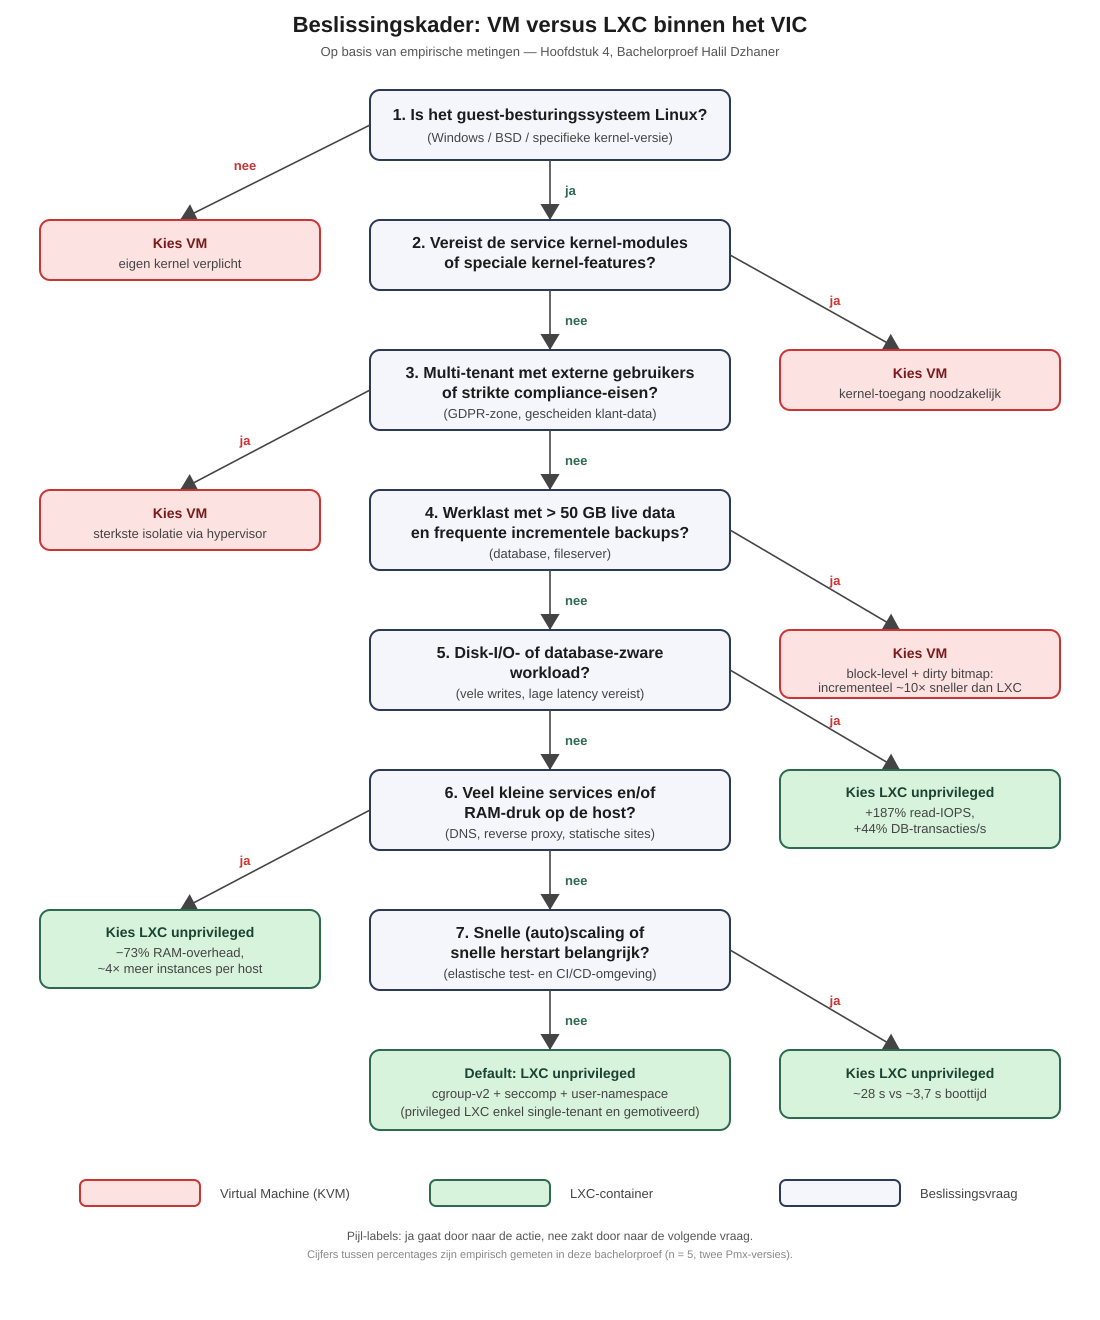
\includegraphics[width=\textwidth]{graphics/decision_tree.pdf}
    \caption{Beslissingskader voor de keuze tussen VM en LXC binnen het VIC, gebaseerd op de empirische metingen uit deze bachelorproef.}
    \label{fig:decision_tree}
\end{figure}

\noindent De redenering achter het kader is als volgt. Vraag~1 vangt de gevallen op waarin een eigen kernel verplicht is (Windows, BSD, of een specifieke Linux-versie); deze workloads passen niet in een LXC-context. Vraag~2 sluit workloads uit die rechtstreekse kernel-modules of -features vereisen die niet via cgroups of namespaces aanstuurbaar zijn (bijvoorbeeld eigen kernel-modules, specifieke FUSE-implementaties of gedeelde TUN/TAP-tunnels). Vraag~3 beoordeelt het isolatie-profiel: zodra externe gebruikers (klanten, studenten in een gedeelde tenant) toegang hebben, of compliance-regelgeving expliciete tenant-scheiding eist, geeft de hypervisor-grens de doorslag voor VM. Vraag~4 weegt het backup-profiel uit Sectie~\ref{sec:resultaten-backup}: bij datasets boven 50~GB met frequente incrementele backups levert de \textit{dirty bitmap} een ordergrootte voordeel op voor VM. Vraag~5 keert de balans om voor I/O- en database-zware workloads, waar de gemeten +175 tot +199~\% IOPS en +43~\% OLTP-throughput een onmiskenbare LXC-voorkeur geven. Vraag~6 valt de typische VIC-situatie voor lichte services aan: bij vele kleine instances en RAM-druk levert het 73~\% lagere geheugen-overhead van LXC een directe consolidatiewinst. Vraag~7 ten slotte vangt elastische scenario's op waarin de boot-tijd telt; LXC start zoals gemeten ongeveer acht keer sneller dan VM. Wie alle vragen met ``nee'' beantwoordt, krijgt LXC unprivileged als veilige default, wat overeenkomt met de huidige VIC-werklasten (DNS, reverse proxy, statische webservers, ontwikkel-omgevingen).

%%=============================================================================
\section{Best practices voor LXC in een VIC-productieomgeving}
\label{sec:best-practices}

Op basis van het beslissingskader en de tijdens de proof-of-concept gemaakte fouten kunnen vijf best practices worden geformuleerd voor een eventuele migratie van VIC-services naar LXC. De eerste betreft de keuze tussen privileged en unprivileged: in een multi-tenant onderwijscontext is unprivileged de standaard, en privileged enkel toelaatbaar wanneer er een aantoonbare functionele noodzaak is en de container in een single-tenant zone draait. De tweede best practice is het expliciet activeren van het AppArmor-profiel \texttt{lxc-container-default-cgns} in de containerconfiguratie; de community-scripts laten dit standaard onaangeroerd, waardoor een hardening-laag onbenut blijft. De derde best practice betreft backup-strategie: voor LXC's met datasets boven ongeveer 20~GB raden wij dagelijkse full backups aan in plaats van het standaard incrementele schema, omdat de file-walking overhead exponentieel toeneemt met het aantal bestanden. De vierde best practice is het systematisch gebruik van \texttt{baseline}-snapshots vóór elke onderhoudsoperatie, wat de gemeten rollback-tijden onder een seconde houdt en menselijke fouten neutraliseert. De vijfde best practice ten slotte betreft de PBS-configuratie: de standaard atime-grace van 24~uur is ongeschikt voor frequent prunen tijdens batch-tests of bij snelle iteratiecycli; voor productie kan deze op 24~uur blijven, maar de garbage collection moet dan minstens dagelijks via een \texttt{systemd}-timer draaien om de chunk-store onder controle te houden.

%%=============================================================================
\section{Beperkingen}
\label{sec:resultaten-beperkingen}

De resultaten van dit hoofdstuk moeten geïnterpreteerd worden met expliciete erkenning van de beperkingen die in Sectie~\ref{sec:beperkingen-validatie} aan bod kwamen. De geneste virtualisatie op één Dell PowerEdge R440 begrenst de absolute meetwaarden, in het bijzonder voor netwerk en schijf. De ``large''-dataset werd op 12~GB beperkt in plaats van de oorspronkelijke 50~GB, omwille van schijfruimte in de geneste opzet. Het aantal herhalingen per prestatie-meting bedroeg vijf, wat statistisch verantwoord is voor $t$-tests maar ruimer mag in een productievalidatie. De security-audit gebruikte de Proxmox-default LXC-configuratie zonder expliciet AppArmor-profiel, wat de gemeten isolatie minimaliseert ten opzichte van een aangepaste productie-opzet. Tenslotte zijn de community-scripts gepind op één commit-hash, wat de reproduceerbaarheid garandeert maar geen uitspraken toelaat over latere versies van diezelfde scripts. Deze beperkingen worden in het volgende hoofdstuk teruggekoppeld aan de aanbevelingen voor toekomstig onderzoek.
